\documentclass[french]{article}
\usepackage[T1]{fontenc}
\usepackage{fullpage}
\usepackage{babel}
\usepackage{hyperref}
\usepackage{graphicx}
\usepackage[justification=centering]{caption}
\usepackage{amsmath}
\usepackage{amssymb}
\usepackage{parskip}

\setlength{\parindent}{0pt}

\hypersetup{
  colorlinks=true,
  linkcolor=black,
  urlcolor=blue
}

\graphicspath{ {./img/} }
\title{%
    \huge Mathfinder  \\
    \bigskip
    \large E5 - Cas pratique \\ 
    Développeur en Intelligence Artificielle,
    titre professionnel enregistré au RNCP - École IA Microsoft by Simplon
    \vfill
    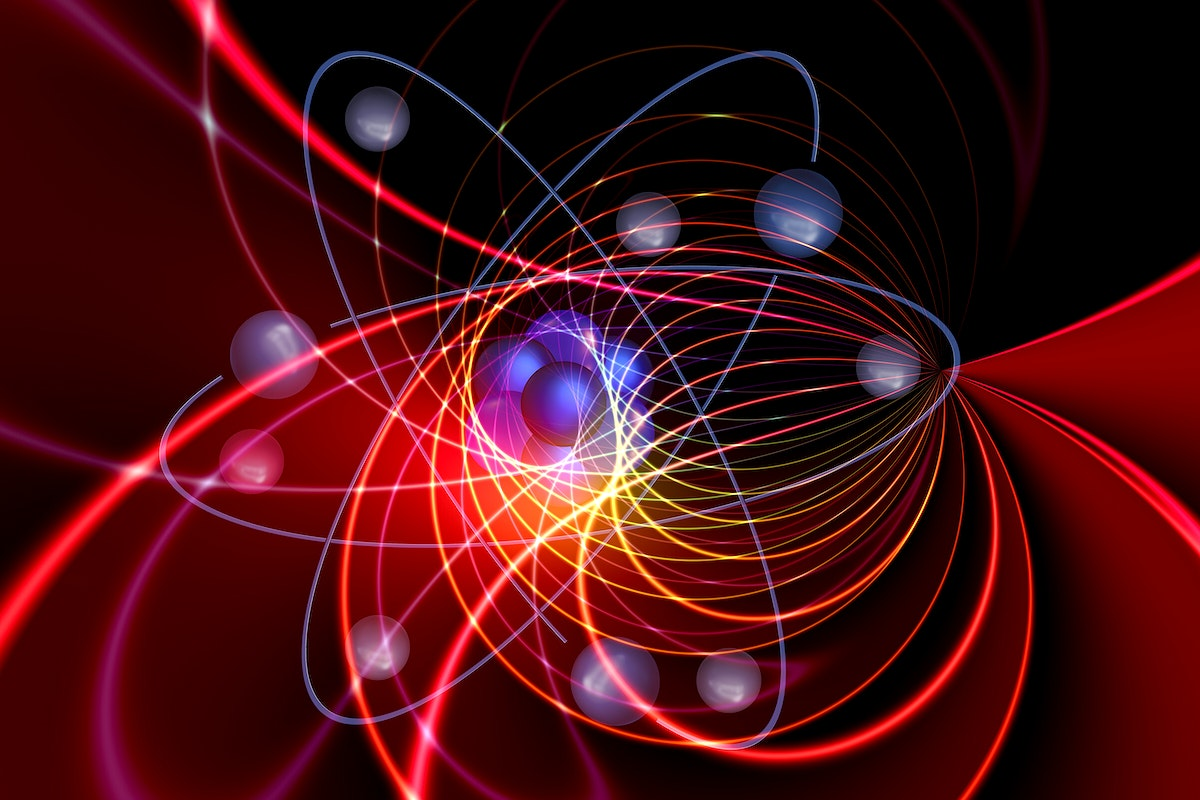
\includegraphics[width=14cm]{physics.jpg} % also works with logo.pdf
    \vfill}
\date{26 février 2024}
\author{par Vincent Papelard}

\begin{document}
    \maketitle
    \pagenumbering{arabic}
    \pagenumbering{gobble}
    \newpage
    \newpage
    \pagenumbering{arabic}

    \section{Contexte}
    Nous sommes les développeurs de Mathfinder, une application web à destination des physiciens. Mathfinder utilise un modèle de régression symbolique afin de calculer la fonction mathématique qui explique le mieux les données issues de leurs observations.

    \begin{figure}[h]
        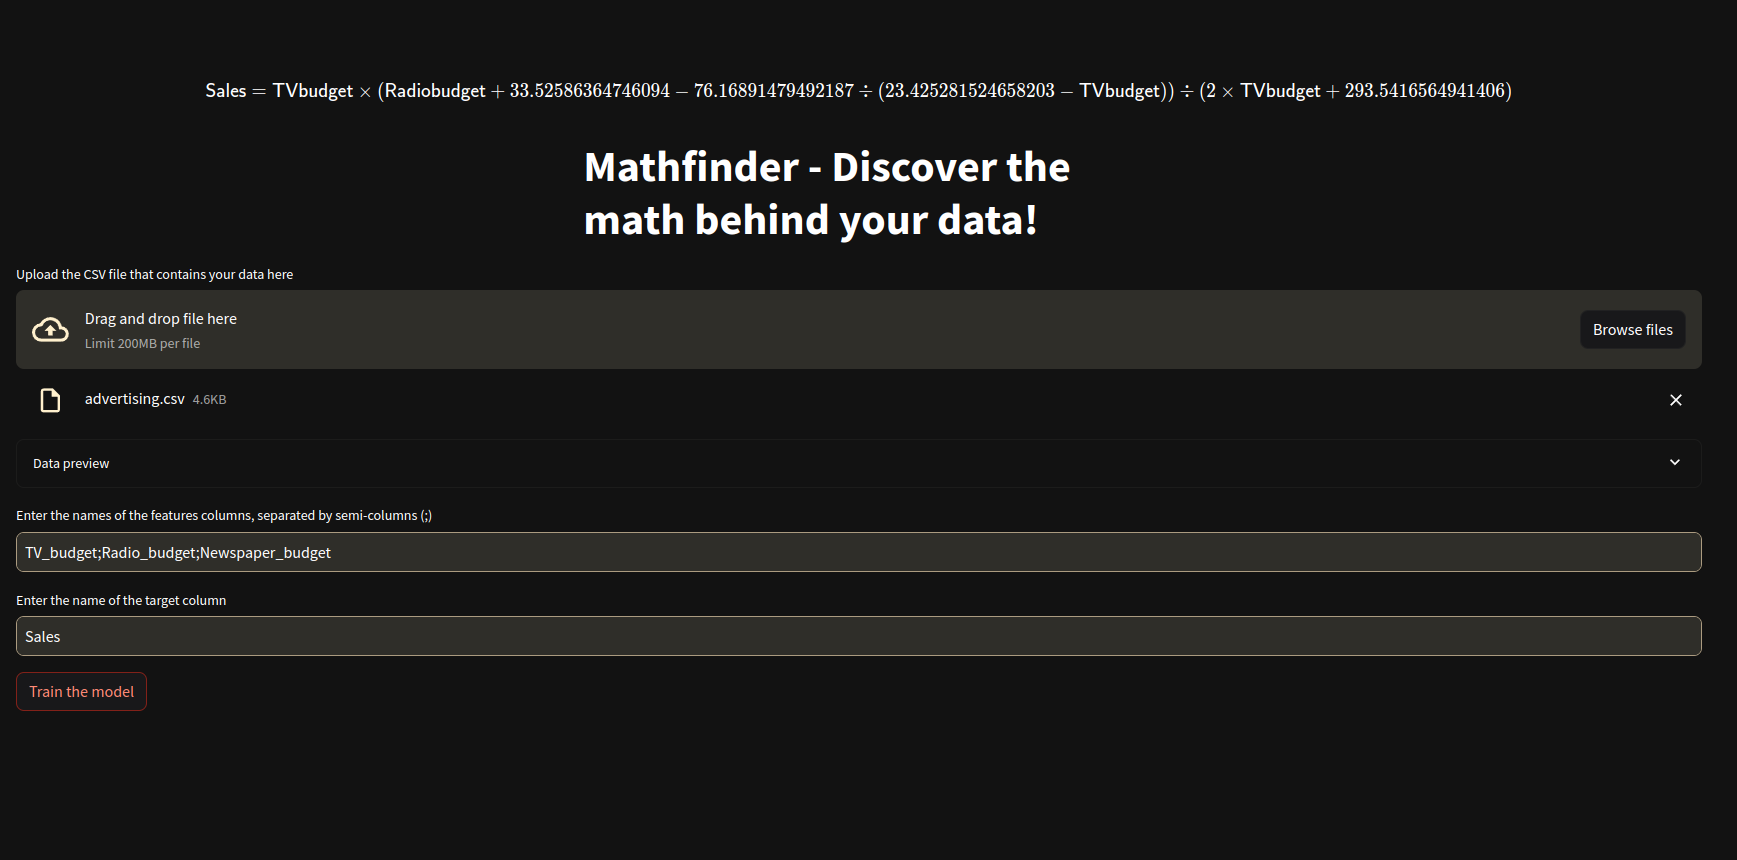
\includegraphics[width=12cm]{appli}
        \centering
        \caption{Mathfinder cherche une formule mathématique qui décrit les relations entre les données que l'on uploade}
        \centering
    \end{figure}

    Le directeur d'une grande université nous contacte. Les chercheurs de cette université ont récemment déployé Mathfinder sur leurs serveurs, mais ils rencontrent des bugs. Insatisfait de notre outil, le directeur exige que nous corrigions ces bugs et nous envoie un descriptif de tous les problèmes rencontrés :
    \begin{itemize}
        \item L'application crash quand on essaie de lui faire prédire les valeurs de deux colonnes ou plus
        \item L'application crash si on ne sépare pas le nom de chaque colonne avec des points-virgules sans espace avant ou après
        \item L'application crash si il manque des valeurs dans certaines colonnes dans le fichier CSV fourni
        \item La fin de la formule affichée à l'écran est tronquée quand elle est trop longue.
    \end{itemize}

    Ce dossier documente deux démarches :
    \begin{itemize}
        \item Le débugging des problèmes rencontrés, de la reproduction du bug à sa documentation sur des tickets GitHub
        \item La mise en place de mécanismes de suivi additionnels afin de rendre notre application plus robuste.
    \end{itemize}
    Le code associé à ce projet est disponible \href{https://github.com/vinpap/mathfinder}{sur GitHub}. Tout au long de ce dossier, des références seront faites à des noms de branche ou identifiants de tickets, avec les liens correspondants. N'hésitez pas à vous y référer !

    \section{Résolution des problèmes}

    \section{Systèmes de suivis additionnels}
    \subsection{Motivations}
    \subsection{Guide d'installation et d'utilisation}

    \section{Conclusion}
\end{document}